
%%%%%%%%%%%%%%%%%%%%%%% file typeinst.tex %%%%%%%%%%%%%%%%%%%%%%%%%
%
% This is the LaTeX source for the instructions to authors using
% the LaTeX document class 'llncs.cls' for contributions to
% the Lecture Notes in Computer Sciences series.
% http://www.springer.com/lncs       Springer Heidelberg 2006/05/04
%
% It may be used as a template for your own input - copy it
% to a new file with a new name and use it as the basis
% for your article.
%
% NB: the document class 'llncs' has its own and detailed documentation, see
% ftp://ftp.springer.de/data/pubftp/pub/tex/latex/llncs/latex2e/llncsdoc.pdf
%
%%%%%%%%%%%%%%%%%%%%%%%%%%%%%%%%%%%%%%%%%%%%%%%%%%%%%%%%%%%%%%%%%%%


\documentclass[runningheads,a4paper]{llncs}

\usepackage{amssymb}
\setcounter{tocdepth}{3}
\usepackage{graphicx}

\usepackage{url}
\urldef{\mailsa}\path|{alfred.hofmann, ursula.barth, ingrid.haas, frank.holzwarth,|
\urldef{\mailsb}\path|anna.kramer, leonie.kunz, christine.reiss, nicole.sator,|
\urldef{\mailsc}\path|erika.siebert-cole, peter.strasser, lncs}@springer.com|    
\newcommand{\keywords}[1]{\par\addvspace\baselineskip
\noindent\keywordname\enspace\ignorespaces#1}

\begin{document}

\mainmatter  % start of an individual contribution

% first the title is needed
\title{Proyecto final de Sistemas de Recuperación de Información}

% a short form should be given in case it is too long for the running head
\titlerunning{SRI}

% the name(s) of the author(s) follow(s) next
%
% NB: Chinese authors should write their first names(s) in front of
% their surnames. This ensures that the names appear correctly in
% the running heads and the author index.
%
\author{Rodrigo García, Jorge Mederos, Javier Valdés}
%
\authorrunning{SRI}
% (feature abused for this document to repeat the title also on left hand pages)

% the affiliations are given next; don't give your e-mail address
% unless you accept that it will be published
\institute{MATCOM, Universidad de La Habana, Cuba\\
\url{http:/matcom.uh.cu}}

%
% NB: a more complex sample for affiliations and the mapping to the
% corresponding authors can be found in the file "llncs.dem"
% (search for the string "\mainmatter" where a contribution starts).
% "llncs.dem" accompanies the document class "llncs.cls".
%

\toctitle{SRI}
\tocauthor{SRI}
\maketitle


\begin{abstract}
El presente trabajo pretende describir el proceso de diseño e implementación de un Sistema de Recuperación de información. El mismo comprende todas las etapas del proceso de recuperación: El procesamiento de la query hecha por un usuario, la representación de los documentos y la consulta, el funcionamiento del motor de búsqueda y finalmente la obtención de resultados. El modelo seleccionado para solucionar el problema es el Modelo Vectorial.
\keywords{Modelo Vectorial, Sistema de Recuperación de Información, Recuperación de Información.}
\end{abstract}


\section{Introducción}
La recuperación de información es un problema existente incluso antes del inmenso crecimiento de la digitalización en la época actual. Se podría afirmar que sus orígenes están en antiguas bibliotecas y centros de documentación en los que se requerían búsquedas bibliográficas de libros o escritos. El objetivo principal de cualquier centro de este tipo es el almacenamiento seguro de la información para satisfacer las necesidades informativas del hombre, de forma veraz, eficiente y pertinente. Esto no ha cambiado con los años, pero las bases de datos, ahora digitales, crecen enormemente en tamaño y se ha hecho necesaria la mejora constante de los sistemas encargados de recuperar la información y satisfacer las necesidades de los usuarios. \\
Los usuarios traducen su necesidad informativa en una consulta adecuada al sistema. Por tanto deben proveer al mismo de un conjunto de términos que expresen semánticamente aquello que desean obtener. El sistema deberá, dada una base de datos y una consulta, proveer al usuario de los documentos más relevantes para sus necesidades. Cómo calcular dicha relevancia varía en dependencia del modelo seleccionado por los desarrolladores de los Sistemas de Recuperación de información.\\
En el presente documento se seleccionaron dos modelos:\\
- El Modelo Vectorial. Ampliamente utilizado en operaciones de recuperación de información, así como en otros campos como la categorización automática o el filtrado de información.\\
- El Modelo RELLENAR AQUÍ


\section{Diseño del sistema}

\subsection*{Procesamiento de textos}



\subsection*{Modelo vectorial}
Una de las ventajas del modelo vectorial es su utilidad para ponderar términos, permitiéndonos crear un ranking ordenado a partir de la relevancia calculada de cada documento, a partir de su similitud con respecto a la query. Además, facilita el proceso de retroalimentación en el que los usuarios juzgan si los documentos recuperados son o no satisfactorios.\\
En este modelo se intenta recoger la relación de cada documento $D_i$, de una colección de $N$ documentos, con el conjunto de las $m$ características de la colección. Formalmente un documento puede considerarse como un vector que expresa la relación del documento con cada una de sus características.

$$ D_i \rightarrow \vec{d_i} = (c_{i1}, c_{i2}, ... , c_{im})$$

El vector identifica en qué grado el documento $D_i$ satisface cada una de las $m$ características. Cada $c_{ik}$ sirve para identificar en qué grado el documento $D_i$ posee la característica $k$. La palabra "característica" puede sugerir un rango bastante amplio de interpretaciones. Podemos concretarlo, por ejemplo, en la ocurrencia de determinadas palabras o términos en el documento.\\

Es necesario entonces procesar como vectores tanto a los documentos como a las consultas para poder trabajar sobre ellos. Una vez obtenidos los vectores, se puede calcular una función de similitud que expresará la relevancia de cada documento. Esta función de similitud se explicará más adelante. \\
Este procesamiento sobre querys y documentos comienza con la tokenización, a partir de la cual se obtienen los términos de los textos y se eliminan caracteres como símbolos de puntiación o espacios. Además, en orden de determinar la similitud de un documento y una consulta, es necesario discernir en qué medida los terminos de los documentos son útiles para la consulta en cuestión. No todas las palabras contribuyen con la misma importancia a la caracterización de un documento. Existen palabras casi vacías de contenido semántico, como los artículos, preposiciones y conjunciones. Pero también son poco útiles aquellas palabras que por su frecuencia de aparición en toda la colección de documentos pierden su poder de discriminación. Por tanto, se aplica sobre los tokens obtenidos, técnicas de eliminación de stopwords (palabras sin contenido semántico), stemming (reducción de palabras con significados similares, pero diferencias en la escritura), lematización (reducir palabras de una misma familia en su $lema$ correspondiente. El $lema$ es la forma que se acepta por convenio como representante de la familia). \\

Una vez obtenidos los términos caracterizadores de la colección de documentos, comienza la fase de vectorización donde se obtendrá el "peso" de los términos en cada documento.\\
para determinar la capacidad de representación de un término para un documento dado, se computa el número de veces que este aparece en dicho documento, obteniéndose la frecuencia del término en el documento ($tf$ por sus siglas en inglés, term frequency). Por otro lado, si la frecuencia de un término en toda la colección de documentos tiene un valor extremadamente elevado, se opta por eliminarlo del conjunto de términos de la colección (eliminación de stopwords), por lo que podría decirse que la capacidad de recuperación de un término es inversamente proporcional a su frecuencia en la colección de documentos. A esto se le conoce como frecuencia inversa del documento ($idf$ por sus siglas en inglés, inverse document frequency).\\

Se tienen las siguientes fórmulas para calcular el $tf$ y el $idf$:

$$
tf_{ij} = \frac{freq(i,j)}{max_l * freq_{ij}}
$$

$$
idf_i = log \frac{N}{n_i}
$$

Luego, el peso $w_{ij}$ de un término $t_i$ en el documento $d_j$ se calcula de la siguiente manera:

$$
w_{ij} = tf_{ij} * idf_i
$$


También es necesario calcular los pesos $w_{iq}$ de las los términos $i$ en las consultas $q$. Esto se consigue de la siguiente forma:

$$
w_{iq} = (a + (1 - a)\frac{freq_{iq}}{max_l freq_{lq}}) * log\frac{N}{N_i}
$$

Finalmente podemos definir la función de similitud mencionada anteriormente y mediante ella, ser capaces de ordenar los documentos según su relevancia. La función de similitud utiliza el coseno del ángulo formado entre los vectores que representan a los documentos y a las consultas.

$$
sim(q_i, d_j) ¡ \frac{\sum_{i = 1}^{n}w_{ij} * w_{iq}}{\sum_{i = 1}^{n}w^2_{ij} \sum_{i = 1}^{n}w^2_{iq} }
$$\\\\


Un modelo de recuperación de información, de forma general, se compone de un cuádruplo [D, Q, F, R(q i , d j ))] donde:\\
◦ D : Es un conjunto de documentos de la colección que conforman el corpus.\\
◦ Q : Es un conjunto de consultas que el usuario realiza al sistema.\\
◦ F : Es un f ramework para modelar los documentos de la colección, las consultas
y sus relaciones.\\
◦ R : Es una función de ranking que asigna a cada par (consulta, documento) un
valor acorde a la relevancia del documento para esa consulta.\\\\

Luego, el modelo vectorial aquí definido, se define formalmente de la siguiente forma:\\
◦ D : Vectores de los pesos asociados a los términos de los documentos.\\
◦ Q : Vectores de los términos asociados a los términos de la consulta.\\
◦ F : Espacio n-dimensional y operaciones entre vectores del álgebra lineal.\\
◦ R : $$ R(q_i, d_j) =
sim(q_i, d_j) = \frac{\sum_{i = 1}^{n}w_{ij} * w_{iq}}{\sum_{i = 1}^{n}w^2_{ij} \sum_{i = 1}^{n}w^2_{iq} }
$$

\subsection*{Modelo RELLENAR AQUÍ}

\subsection*{Interfaz Visual}

\begin{figure}
	\centering
	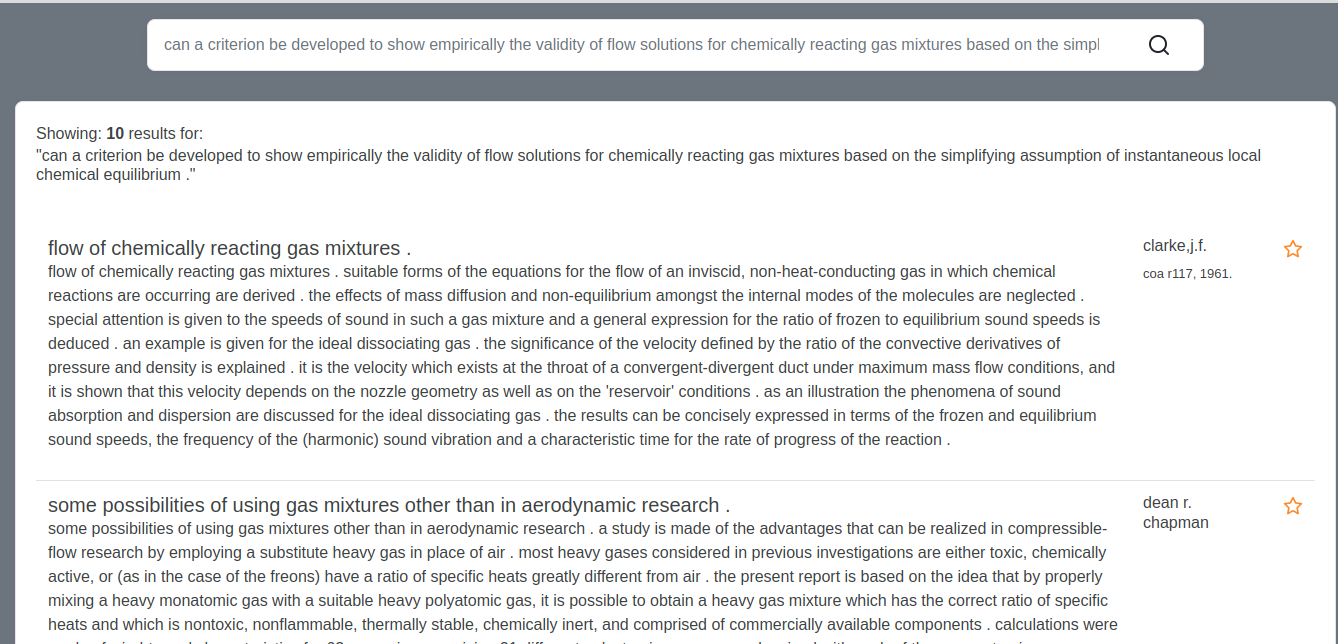
\includegraphics[width=0.7\linewidth]{./visual-1.png}
	\caption{Interfaz visual}
	\label{fig:3}
\end{figure}

En Fig.1 se muestra una captura de la interfaz visual. Al hacer una búsqueda, se muestran los mejores resultados obtenidos por el modelo. Los símbolos de estrellas a la derecha de cada documento constituyen botones que pueden ser pulsados para que el usuario puntúe un documento recuperado a partir de una query. El sistema de feedback permite actualizar los modelos para acomodarse a los usuarios.

\subsection{Detalles de implementación} 




\end{document}
